% {{{1 PRELUDE
\documentclass{beamer}

% Packages
\usepackage[english]{babel}
\usepackage[utf8]{inputenc}
\usepackage[T1]{fontenc}
\usepackage{amsmath,amssymb}

% Custom commands
\newcommand{\R}{\mathbb{R}}

\usetheme{Frankfurt}

\AtBeginSection[]
{
    \begin{frame}
        \frametitle{Outline}
        \tableofcontents[currentsection, hideothersubsections]
    \end{frame}
}

\title[Adaptative point cloud denoising]{Adaptative point cloud denoising}
\author[MEYRON Jocelyn]{MEYRON Jocelyn\\\scriptsize{Tutored by:\\
        ATTALI Dominique, GIPSA-lab\\
        MÉRIGOT Quentin, CEREMADE, Université Paris-Dauphine}}
\institute{GIPSA-lab}
\date{$ 26^{th} $ June 2015}

\begin{document}

\begin{frame}
    \titlepage
\end{frame}

\begin{frame}
    \tableofcontents
\end{frame}

% {{{1 INTRODUCTION
\section{Introduction}

\begin{frame}[allowframebreaks]
    \frametitle{Introduction}
    % \framesubtitle{Introduction}

    What?
    \begin{itemize}
        \item Object of interest: point clouds
        \item Easy to obtain: 3D scanner
        \item Create more complex models: meshes
        \item Issue: measurement error, noise $ \to $ smoothing
    \end{itemize}

    \begin{figure}
        \centering
        \includegraphics[scale=0.25]{img/noise-2d}
        \includegraphics[scale=0.2]{img/elephant-point-cloud}
        \includegraphics[scale=0.2]{img/elephant-mesh}
    \end{figure}

    \newpage
    How?
    \begin{itemize}
        \item Image processing tools unusable: Fourier Transform...
        \item No parametrization: neighbours?
        \item Other idea: mean curvature flow
    \end{itemize}

    \begin{figure}
        \centering
        \includegraphics[scale=0.3]{img/mean-curvature-flow-cube}
    \end{figure}
\end{frame}

\begin{frame}
    \frametitle{Introduction}
    % \framesubtitle{Flot de courbure moyenne}

    Mean curvature flow:
    \begin{itemize}
        \item Move each point of a surface in the direction of the normal by a
            quantity related to the mean curvature at that point
        \item Equivalent to minimize the area of the surface
        \item Smoothing properties
        \item Issue: surface is unknown $ \to $ only samples
    \end{itemize}

    \begin{figure}
        \centering
        \includegraphics[scale=0.25]{img/osculating-circle}
        \includegraphics[scale=0.22]{img/mean-curvature-flow-rabbit}
    \end{figure}
\end{frame}

\begin{frame}
    \frametitle{Introduction}
    % \framesubtitle{Comment?}

    \begin{itemize}
        \item Approximate the area of the surface: union of balls
        \item Minimizing an energy $ E : \R^{dN} \to \R $: gradient descent
        \item Gradient computation: automatic differentiation
            \begin{itemize}
                \item Gradients: variation of the energy when we move each of
                    the points
                \item Overloading of the number type, usual arithmetic
                    operations, functions, chain rule
            \end{itemize}
        \item Other energies: area of the boundary, weighted, anisotropic
    \end{itemize}
\end{frame}

\begin{frame}
    \frametitle{Introduction}
    % \framesubtitle{Objectifs}

    \emph{Objectives}
    \begin{enumerate}
        \item Mean curvature flow on point clouds
        \item Anisotropic mean curvature flow: replace the union of balls with a
            union of convex polyhedra
    \end{enumerate}

    \emph{Applications:}
    \begin{enumerate}
        \item Mean curvature estimation
        \item Smoothing / Denoising
    \end{enumerate}
\end{frame}

% \begin{frame}
%     \frametitle{Introduction}
%     % \framesubtitle{Quelques notions}

%     \begin{definition}[Offset d'un nuage de points]
%         Le $r$-offset d'une nuage de points $ P \subseteq \mathbb{R}^d $ est
%         défini par:
%         $$ P^r = \bigcup_{p \in P} B(p, r) $$
%     \end{definition}

%     \begin{definition}[$\epsilon$-échantillon]
%         Pour une hypersurface $ S $, on dit que $ P \subseteq \mathbb{R}^d $ est
%         un $\epsilon$-échantillon de $ S $ si:
%         $$ \bigcup_{p \in P} B(p, \epsilon) \subseteq S $$
%     \end{definition}
% \end{frame}

% \begin{frame}[allowframebreaks]
%     \frametitle{Introduction}
%     % \framesubtitle{Résultats théoriques}

%     \begin{theorem}[Approximation de l'aire d'une hypersurface]
%         Soit une hypersurface $ S $ de $ \mathbb{R}^d $ et $ P $ un
%         $\epsilon$-échantillon de $ S $, alors:
%         $$ | \frac{Vol^d(P^r)}{2r} - Vol^{d-1}(S) | \leq \frac{\epsilon^2}{2r^2} +
%         O(\frac{\epsilon^4}{r^3}) + O(r^2) $$
%     \end{theorem}

%     \begin{theorem}[Gradient de l'aire]
%         Si $ A = Vol^d(P^r) $ alors en notant $ \nabla_{p_i} A $ la limite
%         suivante:
%         $$ \lim\limits_{\epsilon \to 0} \frac{A(p_1, \ldots, p_{i-1}, p_i + \epsilon
%             \delta p_i, p_{i+1}, \ldots, p_N) - A(p_1, \ldots, p_N)}{\epsilon} $$
%         On a:
%         $$ \nabla_{p_i} A = \int_{B} \frac{x - p_i}{||x - p_i||} dx $$
%         où $ B = \partial B(p_i, r) \cap V(p_i, P) $.
%     \end{theorem}

%     \begin{theorem}[Approximation de la courbure moyenne]
%         Soit une hypersurface $ S $ de $ \mathbb{R}^d $ et soit $ P $ un
%         $\epsilon$-échantillon de $ S $, on a:
%         $$ \nabla_p A \approx 2 r \vec{\kappa}(p) Vol(V(p, P) \cap
%         M) $$
%     \end{theorem}
% \end{frame}

% {{{1 2D
\section{2D case}

\subsection{Problem}
\begin{frame}
    \frametitle{Problem}
    % \framesubtitle{Flot de courbure moyenne}

    Mean curvature flow on point clouds: gradient descent
    \begin{itemize}
        \item Computation of the energy $ E $: area (or perimeter of the boundary) of a union of balls
        \item Gradient computation
        \item Points displacement (Explicit Euler method): $ p'_i = p_i - \tau
            \nabla E (p_i) $ where $ \tau $ is a constant
    \end{itemize}

    \begin{figure}
        \centering
        \includegraphics[scale=0.28]{img/ellipse-balls-15}
    \end{figure}
\end{frame}

\begin{frame}
    \frametitle{Volume computation}
    % \framesubtitle{Flot de courbure moyenne}

    Voronoi diagram with \texttt{CGAL}
    \begin{figure}
        \centering
        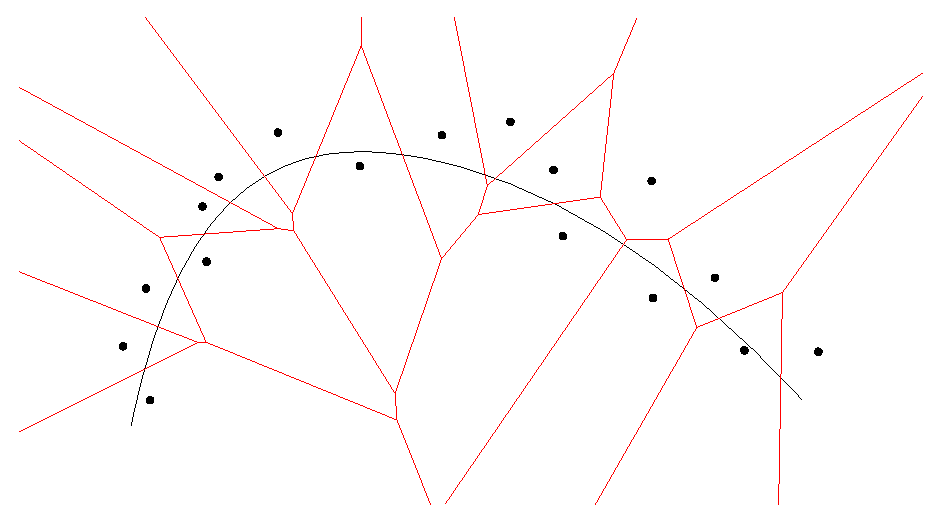
\includegraphics[scale=0.28]{img/voronoi-curve-2d}
        \hfill
        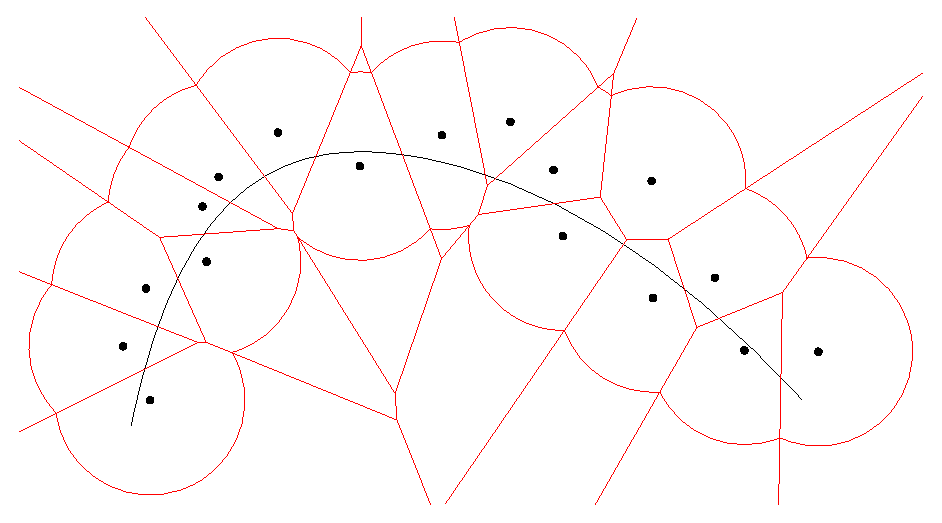
\includegraphics[scale=0.28]{img/voronoi-offset-2d}
    \end{figure}

    Then:
    $$ E \left( \bigcup_p B(p, r) \right) = \sum_p E(V(p, P) \cap B(p, r)) $$
\end{frame}

\subsection{Mean curvature estimation}
\begin{frame}
    \frametitle{Mean curvature estimation}
    % \framesubtitle{Exemples}

    Examples: curvature of an ellipse
    \begin{figure}
        \centering
        \includegraphics[scale=0.3]{img/curvature-ellipse-200-15-area}
        \includegraphics[scale=0.3]{img/curvature-ellipse-200-15-perimeter}
        \caption{E = Area / E = Perimeter of the boundary}
    \end{figure}
\end{frame}

\subsection{Mean curvature flow}
\begin{frame}
    \frametitle{Mean curvature flow}
    % \framesubtitle{Exemples}

    Examples: flow of a noisy ellipse
    \begin{figure}
        \centering
        \includegraphics[scale=0.22]{img/ellipse-200-noised-var-1-area}
        \includegraphics[scale=0.22]{img/ellipse-noised-area-5-01}

        \includegraphics[scale=0.22]{img/ellipse-200-noised-var-1-perimeter}
        \includegraphics[scale=0.22]{img/ellipse-noised-perimeter-7-2}
        \caption{Area / Perimeter of the boundary}
    \end{figure}
\end{frame}

\begin{frame}
    \frametitle{Mean curvature flow}
    % \framesubtitle{Exemples}

    Results:
    \begin{itemize}
        \item Area and perimeter of the boundary: smoothing
        \item Area: creation of holes
    \end{itemize}

    \begin{figure}
        \centering
        \includegraphics[scale=0.22]{img/ellipse-outliers}
        \includegraphics[scale=0.22]{img/ellipse-outliers-area}
        \includegraphics[scale=0.22]{img/ellipse-outliers-perimeter}
        \caption{Point clouds with outliers / area / perimeter of the boundary}
    \end{figure}
\end{frame}

% {{{1 3D
\section{3D case}

\subsection{Problem}
\begin{frame}
    \frametitle{Problem}
    % \framesubtitle{Flot anisotrope}

    Anisotropic flow:
    \begin{itemize}
        \item Union of convex polyhedra
        \item Choice of the polyhedron $ \to $ will influence the directions
            on which points will be moved
    \end{itemize}

    Different methods:
    \begin{itemize}
        \item Naive (approximated): intersection between a Voronoi cell and a
            convex polyhedron
        \item Inclusion-exclusion formulae (approximated)
        \item 3D arrangements (exact?)
    \end{itemize}
\end{frame}

\begin{frame}
    \frametitle{Examples}
    % \framesubtitle{Polyèdres}

    Polyhedra:
    \begin{itemize}
        \item Discretization of a sphere: normal and mean curvature estimation
        \item Cube ($ L_{\infty} $ norm)
        \item Bipyramid ($ L_1 $ norm)
    \end{itemize}

    Intersection computation:
    \begin{itemize}
        \item Voronoi cell and a convex polyhedron
        \item Half-space intersection
        \item Duality
    \end{itemize}

    \begin{figure}
        \centering
        \includegraphics[scale=0.2]{img/circle-cube-inter}
    \end{figure}
\end{frame}

\subsection{Anisotropic flow}
\begin{frame}
    \frametitle{Normal estimation}
    % \framesubtitle{Exemples}

    On a sphere:
    \begin{figure}
        \centering
        \includegraphics[scale=0.22]{img/sphere-polyhedron-200}
        \includegraphics[scale=0.2]{img/sphere-1000}
        \includegraphics[scale=0.2]{img/sphere-sphere-1000-05}
    \end{figure}
\end{frame}

\begin{frame}
    \frametitle{Anisotropic flow}
    % \framesubtitle{Exemples}

    Cube: 10 iterations
    \begin{figure}
        \centering
        \includegraphics[scale=0.4]{img/sphere-cube-0}
        \includegraphics[scale=0.3]{img/sphere-cube-10}
        \includegraphics[scale=0.2]{img/sphere-cube-cube}
    \end{figure}

    Bipyramid: 10 iterations
    \begin{figure}
        \centering
        \includegraphics[scale=0.4]{img/sphere-cube-0}
        \includegraphics[scale=0.2]{img/sphere-bipyramid-10}
        \includegraphics[scale=0.2]{img/sphere-bipyramid-bipyramid}
    \end{figure}
\end{frame}

% {{{1 PERSPECTIVES
\section{Perspectives}

\begin{frame}
    \frametitle{Perspectives}
    % \framesubtitle{Sous-titre}

    \begin{itemize}
        \item Prove the convergence of the area of the boundary towards the mean
            curvature vector
        \item Better understanding of the gradient of the anisotropic flow
        \item Improve the computation in 3D (use 3D arrangements?)
        \item Crystal growth simulation (anisotropic case)
    \end{itemize}
\end{frame}

% \plain{Merci!}
\begin{frame}
    \begin{center}
        \huge{Thank you!}
    \end{center}
\end{frame}

\end{document}

% vim: set spelllang=fr :
